% Chapter 3

\chapter{The COMPASS experiment at CERN} % Chapter title

\label{ch:exp} % For referencing the chapter elsewhere, use \autoref{ch:name}

In this chapter a description of the COMPASS experiment is provided. The general features of the spectrometer are given in Section. \ref{sec:specgen}. The beam and target are presented in Section. \ref{sec:beam}. The descriptions of the detectors used for the tracking and the ones used for the particle identification are respectively done in Section. \ref{sec:track}. The trigger system is discussed in Section. \ref{sec:trigger}. Eventually the last sections deal with data acquisition and reconstruction.

%----------------------------------------------------------------------------------------

\section{General Overview}\label{sec:specgen}

COMPASS is a high energy, high rate and fixed target experiment at the Super Proton Synchrotron (SPS) at CERN. It is dedicated to the study of hadron structure and hadron spectroscopy with high intensity muon and hadron beams.

The COMPASS spectrometer (as in Fig. \ref{pic:apparatus}) covers a large kinematic domain : $Q^2$ values up to 100 (GeV/c)$^2$
and x values down to $10^{-5}$ for an incoming muon beam of 160 Gev/c.

The apparatus is divided in three parts : the first part is dedicated to the detection of the incoming beam and is located upstream the target location. The second and third parts are downstream of the target and are totalizing a length of 50 meters. The second part called the \textit{Large Angle Spectrometer} (LAS) is built around the magnet SM1.
The LAS has been designed to provide a 180 mrad acceptance. The \textit{Small Angle Spectrometer} (SAS), built around the magnet SM2, measures the particles emitted at small angles ($\pm$30 mrad).

In 2016, the data taking was performed with a 160 Gev/c muon beam scattering on a liquid H$_2$ target.

\begin{figure}[!h]
  \centering
	\subfloat[LAS]{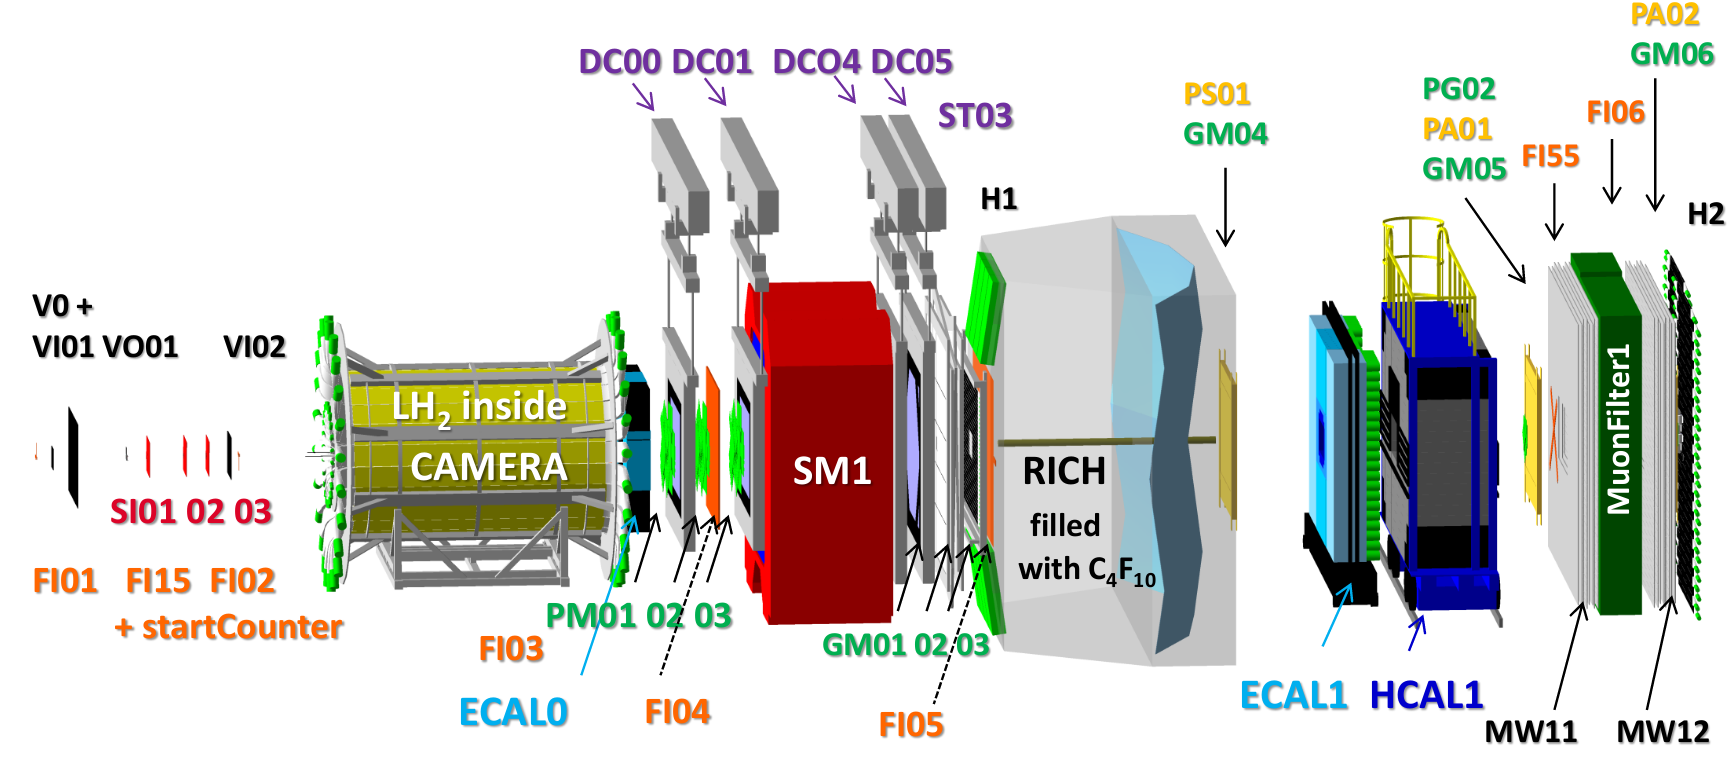
\includegraphics[scale=0.17]{./gfx/Apparatus1.png}}
  \subfloat[SAS]{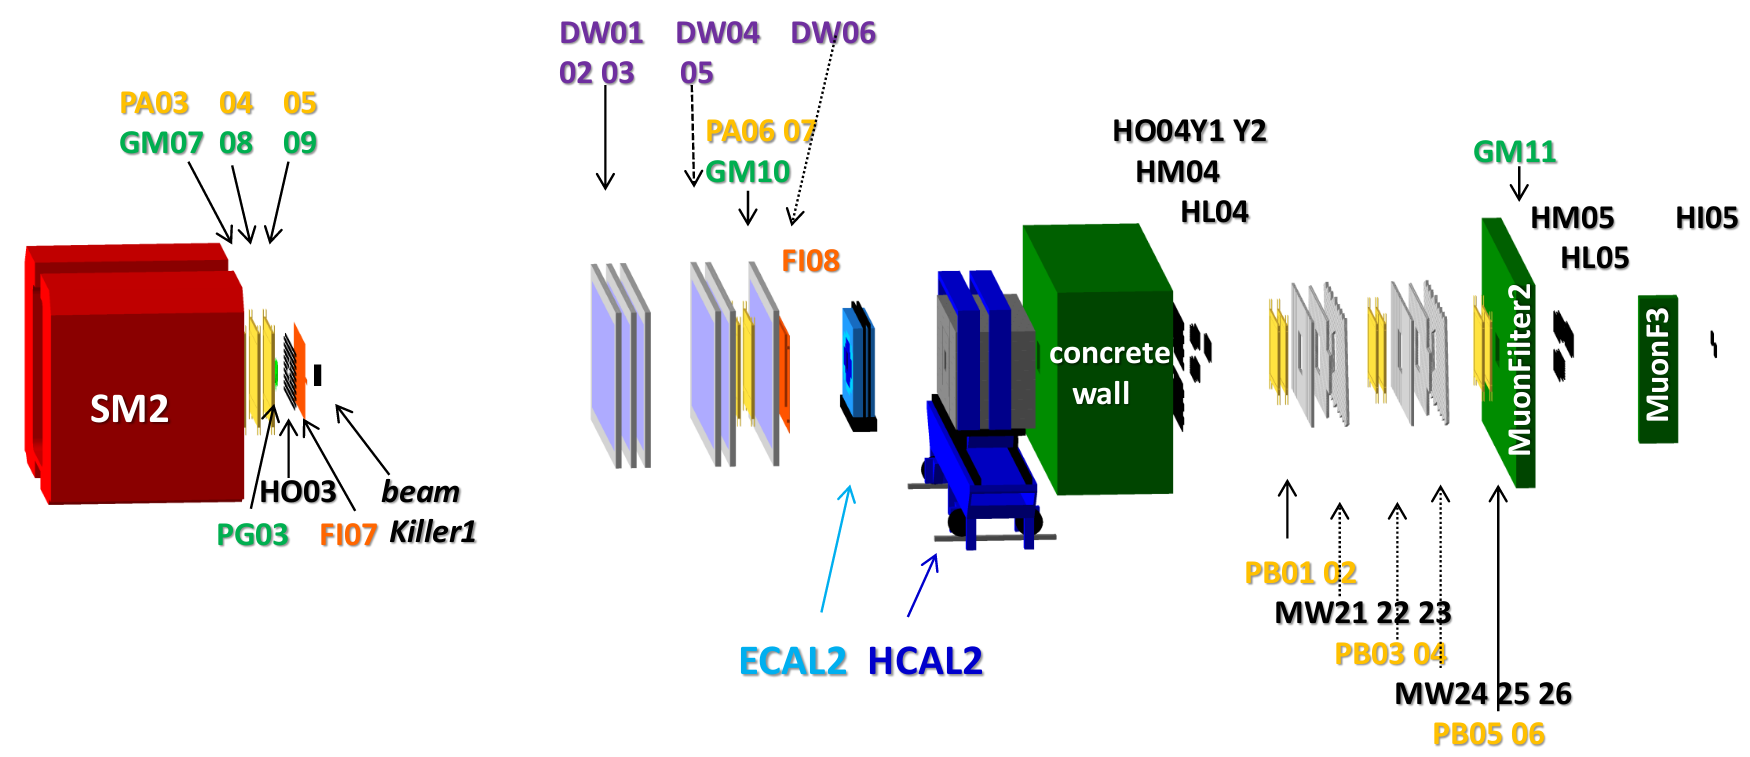
\includegraphics[scale=0.17]{./gfx/Apparatus2.png}}
	\caption{COMPASS 2016/2017 muon setup side view. Taken from \cite{NIM}.}
	\label{pic:apparatus}
\end{figure}

%----------------------------------------------------------------------------------------

\section{Beam}\label{sec:beam}

The muon beam used by COMPASS is obtained from a primary proton beam accelerated in the SPS up to 400 GeV/c. The proton beam interacts with T6 target, a 50 cm thick beryllium target, producing pions and kaons. The spill time, which is the time period window within which the proton beam is delivered to the T6 target, is of 4.8 s. The produced hadrons are transported in a 600 m long channel of the M2 beamline \ref{}. During this time, 5\% of the pions are decaying into muons and neutrinos. Remaining pions and a large amount of the muons obtained from the decay are transported until the muons are focused and the hadrons stopped by a hadron absorber. A system of magnets is then used to select and focus
the muons of 160 GeV/c. The muons coming from the $\pi \rightarrow \mu\nu$ weak channel decay are polarized ; nevertheless this feature is not used in this analysis.

In the experimental area, the beam has transverse dimensions of $\sigma_x \times \sigma_y \sim 8 \times 8 $ mm$^2$ and an angular divergence of $\sigma_{\theta_x} \times \sigma_{\theta_y} \sim 0.5 \times 1 $ mrad$^2$. In mean, at each spill, $2.10^8$ muons enters the experimental area. Along with the beam is a large muon halo that extends transversely up to several meters of distance with respect to the beam line. The intensity of this halo decreases with the distance. The high intensity halo near the beam line is measured by a $30 \times 30$ cm$^2$ dedicated veto counter with a 4 cm diameter central hole. It represents $\sim$ 16\% of the muon beam. The far halo or low intensity halo is measured by a large veto counter of $? \times ?$ cm$^2$ with a central hole of $30 \times 30$ cm$^2$. It represents $\sim$ 7\% of the muon beam.

\subsection{The Beam Momentum Station}

The Beam Momentum Station (BMS) is used for the determination of the incident muon momentum. It consists of six scintillators hodoscopes (BM01-BM06) located symmetrically upstream and downstream a bending magnet (B6 : three consecutive dipole magnets) surrounded by four quadrupoles (Q29-Q32). The BMS is illustrated in Fig. \ref{pic:BMS}.

The BMS system was designed to measure the momentum of more than $10^8$ individual particles per spill with a relative precision of 0.5\%. To eliminate the ambiguities in the reconstruction of particle trajectories, their time of transit is measured with a resolution of 50 ps.

\begin{figure}[!h]
  \centering
	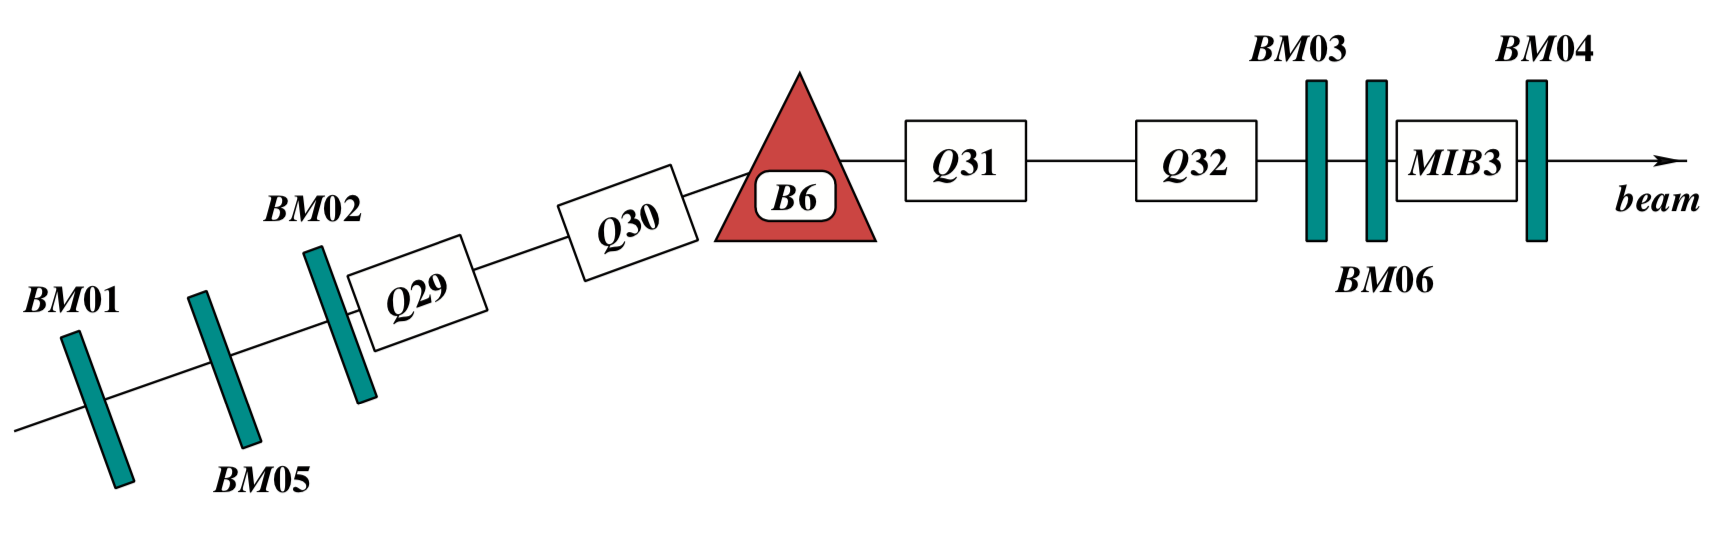
\includegraphics[scale=0.5]{./gfx/BMS.png}
	\caption{Layout of the Beam Momentum Station for the COMPASS muon beam. Taken from \cite{NIM}.}
	\label{pic:BMS}
\end{figure}

%----------------------------------------------------------------------------------------

\section{Target}

\begin{figure}[!h]
  \centering
	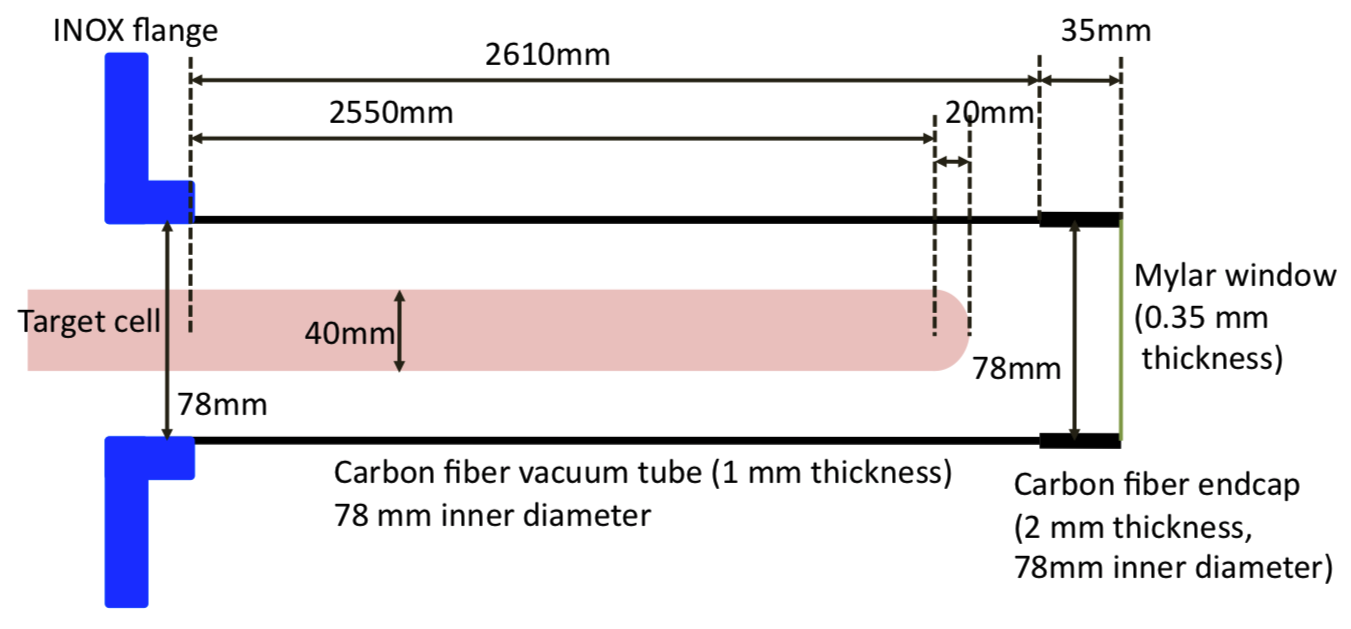
\includegraphics[scale=0.3]{./gfx/Target.png}
	\caption{Target geometry for the 2016/2017 setup.}
	\label{pic:Target}
\end{figure}

The target is one monolythic 2.5 meter long cylinder with a radius of 2 cm and contains lH$_2$ (Fig. \ref{pic:Target}). The main component of the target system is the refrigerator system that is used to conserve the target temperature between 55 and 90 mK.

%----------------------------------------------------------------------------------------

\section{Tracking Detectors}\label{sec:track}

The \textit{Large Angle Spectrometer} (LAS) and \textit{Small Angle Spectrometer} (SAS) are each equipped with different type of tracking detectors. Depending on the direction coverage area of each detectors they are classified as :
\textit{very small area trackers}, \textit{small area trackers} and \textit{large area trakers}

\subsection{Very small area trackers}

The very small area trackers cover the transverse beam size up to $\sim$ 3 cm. In this region the particle rate is very
high ($10^5$/s/mm$^2$ in the center of the muon beam) hence the tracking detectors must have an excellent time and position
resolutions.

The scintillating fibers detectors are the smallest one in the spectrometer and their size is comprised between $\sim$ 16 cm$^2$
and 144 cm$^2$. The best characteristic of this kind of detectors is their time resolution of approximately 500 ps. All along the
apparatus there are 9 stations composed by two or three scintillating fiber detectors. The third detector is always pivoted by 45°
with respect to the others.

The silicon detector size is 30 cm$^2$ with a space and time resolution of $\sim$ 10 $\mu$m and $<$ 2.5 ns. The measurement
of the incoming muon beam track is improved with these detectors in addition to the BMS. The 3 silicon detectors stations are
located upstream the target. The stations are each composed by two silicon detectors, the second one being rotated by 5° with
respect to the other.

\subsection{Small area trackers}

The radial region between 2.5 cm and 20 cm is covered by small trackers. Two types of gaseous detectors which combine a high rate capability ($\sim$ 10$^4$/s/mm$^2$) and good spatial resolution ($<$ 100 $\mu$m) with minimal material budget are used : Micromegas (MICRO MEsh GAseous Structure) and GEM (Gas Electron Multiplier) detectors.

A GEM is a thin polyimide foil (50 $\mu$m) with Cu cladding on both sides, into which numerous microholes ($\sim$ 10$^4$/cm$^2$) with a diameter of 70 $\mu$m has been chemically etched using lithographic techniques. The COMPASS GEM detection principle is shown in Fig. \ref{pic:GEM} : it consists of three GEM amplification stages separated by thin grids of 2 mm height. A high voltage (several 100 V) is applied to each foil to generate the avalanche multiplication of the electron through the holes. The fast signal is induced by the electron cloud emerging from the last GEM foil on an anode segmented into two sets of 768 orthogonal strips (pitch of 400 $\mu$m). A GEM station is composed by 2 detectors oriented by 45° relatively to each other. All in all there are 11 stations, all located at SAS. The active area for the GEM is $31 \times 31$ cm$^2$ and the central area of 5 cm diameter can be activated to align the detector with low intensity beams. The detectors efficiency is $\sim$ 97\% with a spatial and time resolution of respectively $\sim$ 70 $\mu$m and 12 ns.

\begin{figure}[!h]
  \centering
	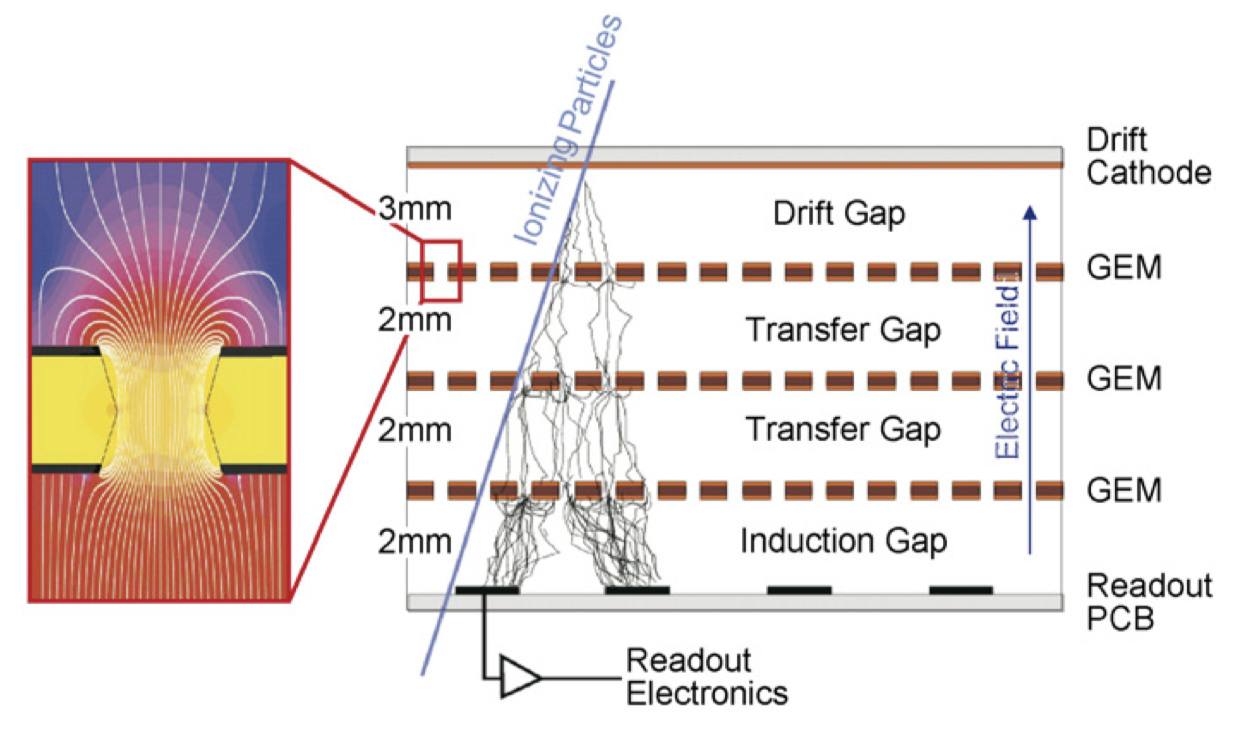
\includegraphics[scale=0.5]{./gfx/GEM.png}
	\caption{COMPASS GEM detection principle. Taken from \cite{NIM}.}
	\label{pic:GEM}
\end{figure}

There are 3 Micromegas stations, located at LAS. They are composed by four detectors each with different directions : horizontal (X), vertical (Y), and two (U,V) rotated by $\pm$45° with respect to the vertical. Each plane has an active area of $40 \times 40$ cm$^2$ with a deactivated central zone of 5 cm diameter. The principle of the detector is explained in Fig. \ref{pic:MM}. The particle ionizes the gas in the conversion gap, the produced electrons drift in a moderate field of 1.5 kV/cm to prevent secondary ionization, towards the amplification gap. The field in the amplification zone is large enough to accelerate the electrons to produce an avalanche. The conversion and amplification gaps are separated by a \textit{micromesh} which collects the positive ions produced during the avalanche in a short period of time ($<$ 100 ns). This feature is possible because of the small width of the gap ($\sim$ 100 $\mu$m). All Micromegas detectors operate with a detection efficiency of 98\% and with a spatial resolution of less than 100 $\mu$m.

\begin{figure}[!h]
  \centering
	\subfloat[]{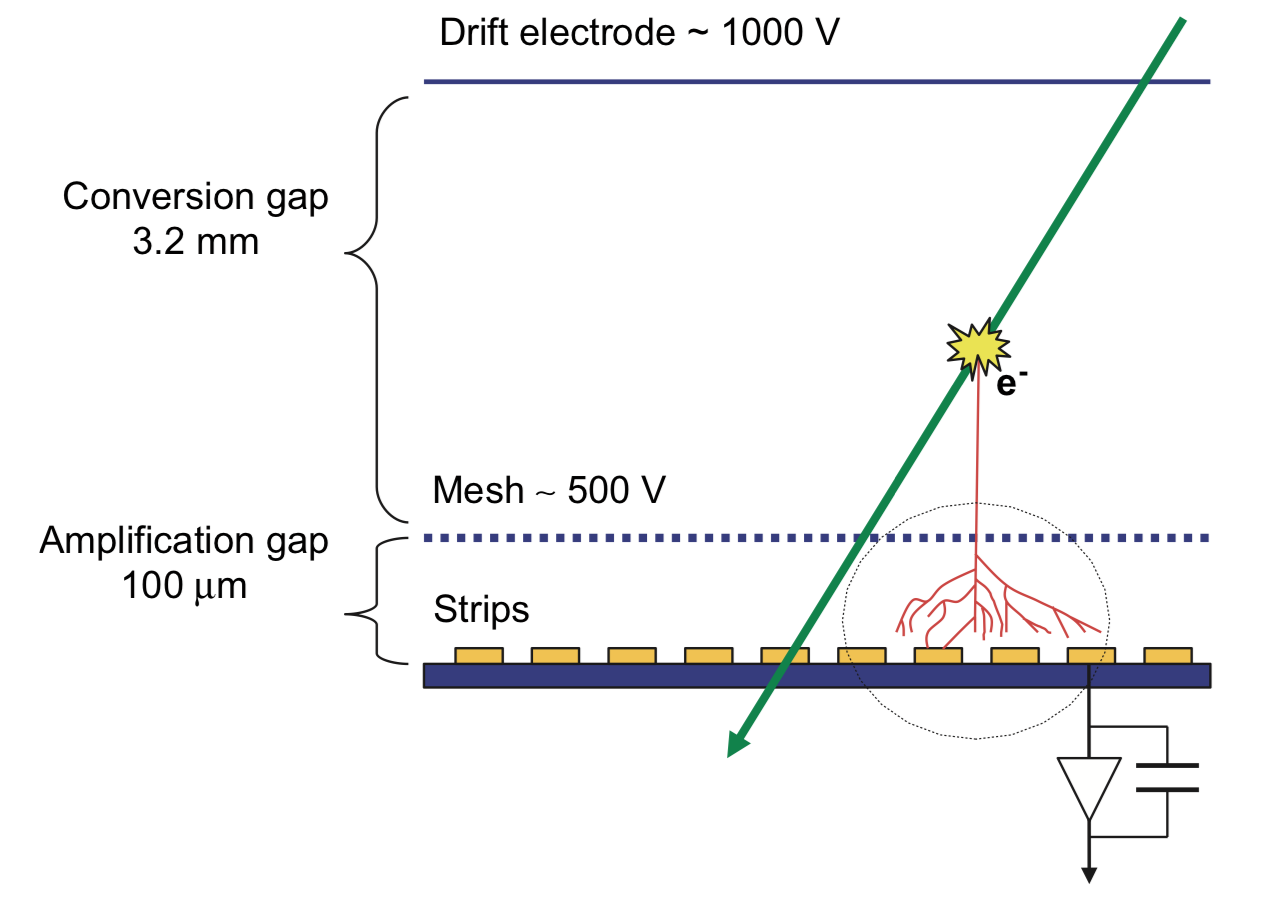
\includegraphics[scale=0.35]{./gfx/MM1.png}}
  \subfloat[]{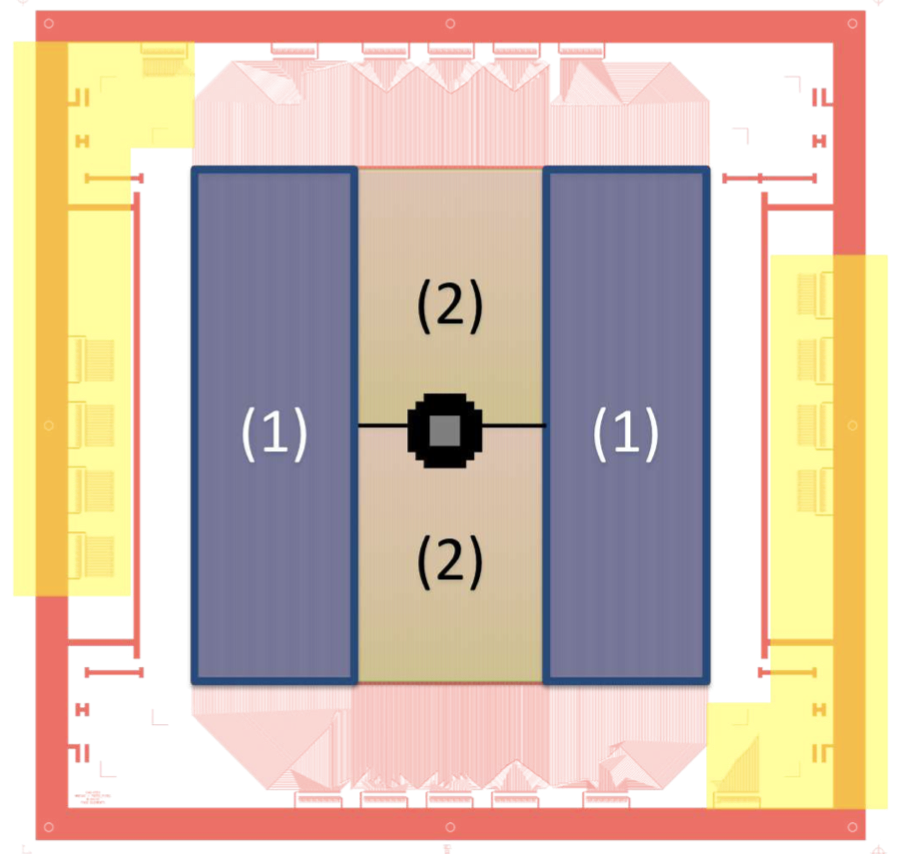
\includegraphics[scale=0.35]{./gfx/MM2.png}}
	\caption{(a) COMPASS MicroMegas detection principle. (b) MicroMegas detector. Taken from \cite{NIM}.}
	\label{pic:MM}
\end{figure}

\subsection{Large area trackers}

The large area trackers cover all the spectrometer acceptance with a good spatial resolution. As the particle rate in the region
covered by the large area trackers is small in comparison to the central region (10$^2$/s/mm$^2$), the use of detectors such as
drift chambers (DCs) \cite{}, straw drift tubes \cite{} and multiwire proportional chambers (MWPCs) is possible. These detectors
have large active size area ($\sim$ m$^2$) with a central dead zone of few cm$^2$.

Each DC consists of eight layers of wires with four different inclinations : horizontal, vertical and rotated $\pm$20° with respect
to the vertical direction. Two consecutive planes with the same inclination are staggered by 3.5 mm to disimbiguate left-right and
the ordering of the planes with different orientations is such to minimize the fake track combinations. Two of the DC are located before
SM1 and have an active area of $180 \times 127$ cm$^2$ ; the third one is located downstream SM1 and has a larger active area of $204 \times 204$ cm $^2$.
All these DCs have a central dead zone of 30 cm. The central dead zone can be activated for alignment needs with a low intensity beam.
The average resolution of a DC is 270 $\mu$m and the efficiency above 95\%.

A straw detector station consists in 3 straw detectors with different orientations : horizontal, vertical and rotation by 10° with respect
to the vertical. Five stations in total are located vetween SM1 and SM2. Each detector is composed by two layers of straw tubes with the
same orientation. The straw tubes consist in two layers of thin plastic film, one coated with carbon loaded Kapton, the other one with
aluminised Kapton foil. The active area for the straw detector is $320 \times 280$ cm$^2$ and have a central dead zone of $20 \times 20$ cm.
The average resolution is of 190 $\mu$m.

There are three types of MWPC in COMPASS, each one of them having its own quantity of layers. The A-type has three vertical layers and two tilted
by $\pm$ 10° with respect to the vertical direction. The A*-type has four layers, 3 identical to the A-type and the last one oriented horizontally.
Both have an active area of $178 \times 120$ cm$^2$. The B-type has two double layers detectors with opposite orientation fixed together. Of these
four layers only three are read out : the vertical and tilted ones. The active area is of $178 \times 180$ cm$^2$. All layers have a wire length of
about 1 m, a wire diameter of 20 $\mu$m and a pitch of 2 mm and are enclosed on both sides by graphite-coated Mylar foils. The central deadzone of each
detector increases with respect to the detector position, from 16 to 22 cm. The average spatial resolution of the MWPC is of 1.6 mm.

%----------------------------------------------------------------------------------------

\section{Particle Identification}

The particle detection is performed by the combination of several detectors. A RICH detector allows to separate hadrons between pions, kaons and protons
at high intensity environment. Two types of calorimeters are used to measure the energy of the hadrons, photons and electrons : hadrons calorimeters
(HCAL1 and HCAL2) and electromagnetic calorimeters (ECAL1 and ECAL2). Two muon wall detectors (MW1 and MW2) are performing muon identifications and
consist of tracking detectors combined with a hadron absorber. While the RICH will be further described in a dedicated chapter (Chap. \ref{}), the other
identification detectors will be briefly described in the following subsections.

\subsection{Hadron Calorimeters}

A hadron calorimeter allows to separate hadron and muon tracks depending on the energy deposit. Contrary to the hadron which deposit almost all its energy
via a hadronic shower, the muon only deposit a small energy fraction. The signal measured is used to determine the hadron energy by a linear relation \cite{}.
HCAL1 and HCAL2 are simple calorimeters with a modular structure with iron and scintillator plates and are located before the muon filters. Their efficiency
depends on the energy : for HCAL1 for hadrons with momenta above 5 GeV/c it is almost constant and close to 100\% when for HCAL2 the same efficiency is reached
for hadrons with momenta above 10 GeV/c.

\subsection{Electromagnetic Calorimeters}

The electromagnetic calorimeters are used to identify electrons and detect photons. ECAL1 and ECAL2 are formed by blocks of lead glass connected to photomultipliers
with light guides. An electromagnetic shower is initiated when the incoming electrons of photon go through the calorimeter. This electromagnetic shower produces
Cherenkov radiation inside the lead glass and this light intensity is proportional to the energy deposited.

\subsection{Muon Wall Detector}

The muon wall detectors MW1 and MW2 consist of a set of tracking stations and a hadron absorber. For MW1 it is a 60 cm thick iron wall and for MW2 a 2.4 m concrete wall.
Muons passing through the MW detector are detected before and after the absorber while all other tracks are stopped.

%----------------------------------------------------------------------------------------

\section{The Triggering System}\label{sec:trigger}

The triggering system \cite{} has the task to select physical event candidates in a high rate environment. It is composed by scintillating hodoscope stations, scintillator veto stations to exclude halo muons and calorimeters to select event with hadron production.

\begin{table}[!h]
  \caption{COMPASS triggers with the muon beam in 2016.}
  \label{tab:kinvar}
  \centering
  \begin{tabularx}{7.5cm}{cc}
    \hline
    \hline
    Trigger name & Components \\
    \hline
    \hline
    Middle Trigger (MT) & H4M, H5M \\
    Ladder Trigger (LT) & H4L, H5L \\
    Outer Trigger (OT) & H3O, H4O \\
    LAS Trigger (LAST) & H1G, H2G \\
    Pure Calo Trigger (CT) & HCAL1, HCAL2 \\
    \hline
    \hline
  \end{tabularx}
\end{table}

Depending on the event kinematics two different algorithms are used to determine the scattered muon kinematics. When the angle of the scattering muon is large enough (Q$^2$ > 1 (GeV/c)$^2$) to be measured by using only the hodoscope stations, the trigger signals are built using the vertical pointing algorithm (Fig. \ref{pic:triglogic}).

\begin{figure}[!h]
  \centering
	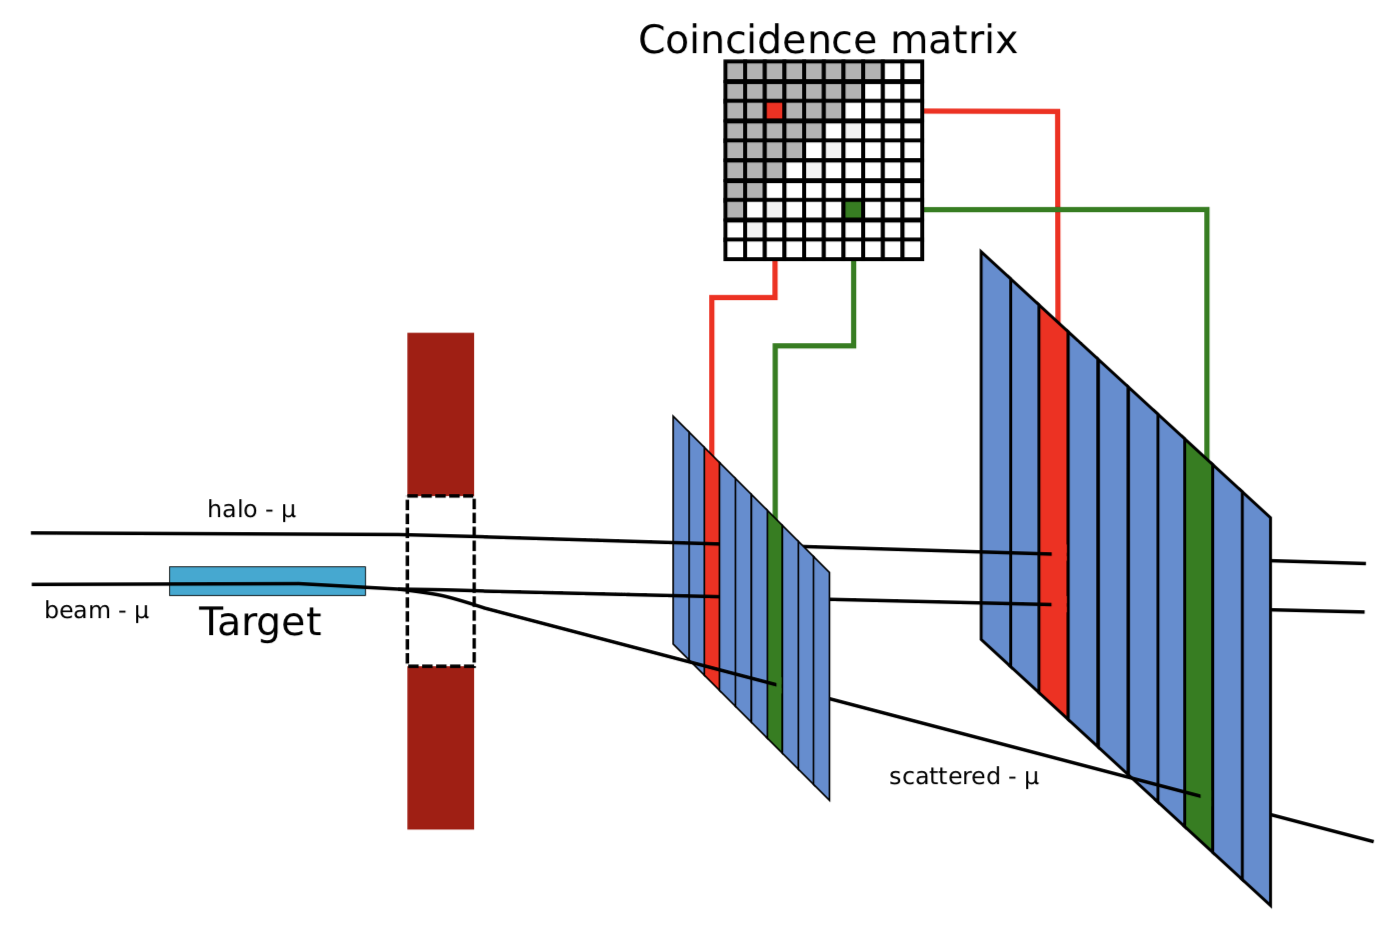
\includegraphics[scale=0.5]{./gfx/TriggerLogic.png}
	\caption{Concept of the trigger for quasi-real photoproduction with high energy loss. The scattered muon leads to a coincidence in the activated area of the coincidence matrix while the halo muon fails to do so. In addition, a minimum hadron energy can be required in the calorimeter. Taken from \cite{NIM}.}
	\label{pic:triglogic}
\end{figure}

The angle ($\theta_x,\theta_y$) of the scattered muon is determined by using two hodoscopes with horizontal strips located at different positions along the beam direction and the vertical component $\theta_y$ is determined. If $\theta_y$ is compatible with the target position the trigger system validates the event. The $y$-$z$ plane is selected since the particle track is not bent by the dipole magnet in the y-direction. In the case where the scattering angle of the muon is too low to be measured (Q$^2$ < 1 (GeV/c)$^2$), the bending angle of the magnet is used to determine $\theta_x$ and to perform an energy loss criterion to fire the trigger. This is possible since the muon energy loss $\nu$ is translated into a deflection by the magnetic dipole field. In the low Q$^2$ region the information coming from the hodoscopes is not enough to tag the event as there are several background processes in the scattered muon signal (elastic scattering off target electrons, quasi-elastic radiative scattering off target nuclei). To improve the trigger signal, an energy deposit in the HCALs larger than 5.4 GeV can in addition be required. In the particular case where any scattered muon is detected, it is still possible to determine if an elastic interaction has occured. If a large deposit of energy viz. above 16.2 GeV is registered in any HCAL, the event will fire the trigger.

The kinematic range covered by the trigger system us shown in Fig. \ref{pic:trigger}. The trigger system is optimized to select \textit{quasi-real photon} and DIS events. The quasi-real photon events correspond to the low Q$^2$ region ($\sim$0) and they will be detected by the \textit{ladder} (LT) trigger. A DIS event is characterized to have higher Q$^2$ values. The \textit{middle} (MT) trigger is in charge of the DIS events with small to moderate Q$^2$. The \textit{outer} (OT) and \textit{large angle spectrometer} (LAST) triggers are designed to detect DIS events with high Q$^2$.

\begin{figure}[!h]
  \centering
	\subfloat[]{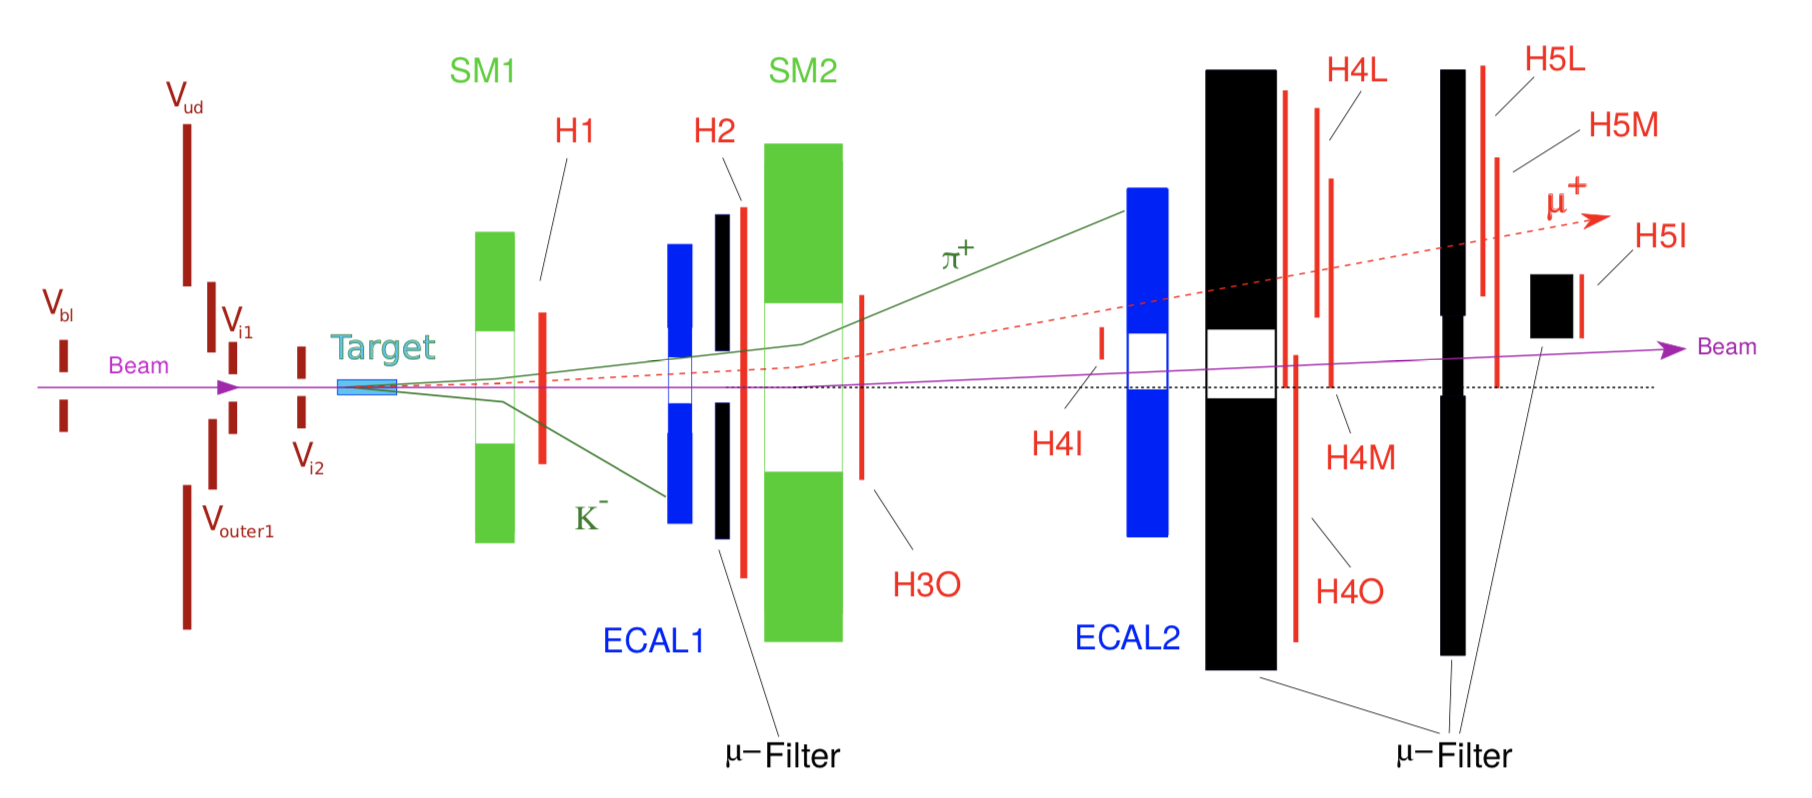
\includegraphics[scale=0.4]{./gfx/TriggerSys.png}}
  \subfloat[]{\includegraphics[scale=0.30]{./gfx/TriggerCov.png}}
	\caption{(a) Main elements of the trigger system. (b) Trigger system kinematic coverage.}
	\label{pic:trigger}
\end{figure}

%----------------------------------------------------------------------------------------

\section{Data Acquisition}

The data acquisition system (DAQ) \cite{} is in charge of managing the information coming from more than 250000 spectrometer electronic channels to be sent to permanent storage.
At COMPASS the typical event size is 45 kB at a trigger rate of about 10 kHz. The pipeline used in the DAQ is illustred in Fig. \ref{pic:DAQ}. First the analog signals are coming from
the detectors are preamplified, then they are digitized directly at the front-end by Analog to Digital Converters (ADCs) or Time to Digital Converters (TDCs) according to the type
of detectors the front-ends are coupled to. The data are then transferred to the readout driver modules CATCH (COMPASS Accumulate, Transfer and Control Hardware) of GeSiCA (GEM and
Silicon Control and Acquisition) upon the arrival of a trigger signal provided by the Trigger Control System (TCS). CATCH and GeSiCA combine the data from up to 16 cards (ADC or TDC)
and transmit them via an optical S-Link to the computers named \textit{Readout Buffer} (ROBs, maximum through output 160 MB/s) where they are stored in 512 MB spill buffer cards.
During the 4.8 s of beam time the data are written to memory, during the rest of the full SPS cycle (12 s) they are read through a PCI interface. In this way the required bandwidth
is reduce by a factor of three. The events are written to multiple 1 GB large files (chunks) labeled by the run number and their consecutive chunk number. Finally the data are transferred
to the CERN central data recording facility (CASTOR).

\begin{figure}[!h]
  \centering
	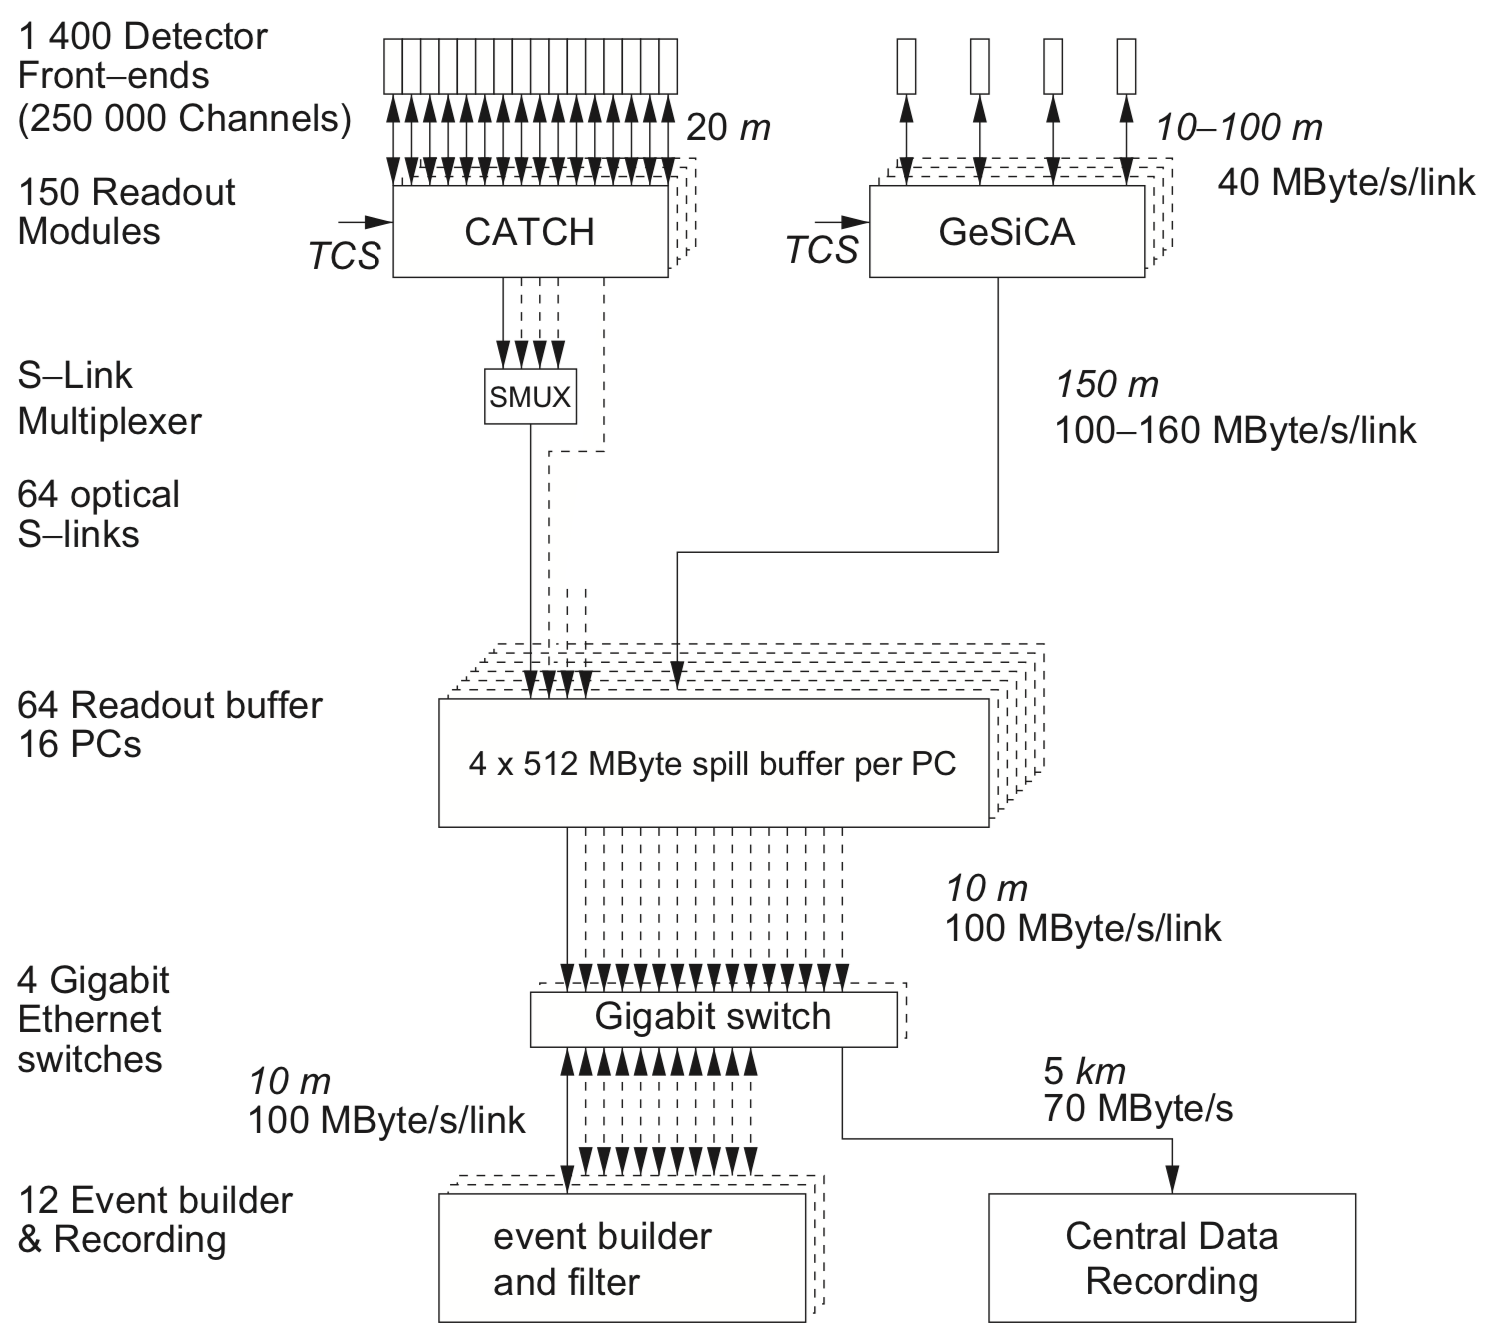
\includegraphics[scale=0.4]{./gfx/DAQ.png}
	\caption{General architecture of the DAQ system. Digitized data from the detector front-end are combined on the CATCH and GeSiCA modules. The storage of the data during the spill and the event building is performed locally. The data are recorded at the CERN computing center. Taken from \cite{NIM}.}
	\label{pic:DAQ}
\end{figure}

%----------------------------------------------------------------------------------------

\section{Event Reconstruction}

The offline reconstruction of the events stored in CASTOR is performed by the COMPASS software CORAL \cite{}. CORAL is also used for the reconstruction of events generated by the Monte-Carlo
simulation TGEANT (see Chapter\ref{ch:MC}). CORAL is written in C++ and has a modular structure. The scheme of the steps followed by the reconstruction program are shown in Fig. \ref{pic:CORAL}. First the
information on the fired detectors channels is extracted. This is known as decoding and in the MC case digitization. In general there are more than one detector channels fired by the same
particle. In that case a clustering algorithm is applied viz. the neighbouring detector channels that were fired are groupes together and the coordinate of the cluster in the apparatus reference
system is computed. At this stage the detector calibration and position are used to extract the information. The CORAL output is stored in a ROOT Tree called mDST (mini Data Summary Tape).

The physics informations are extracted from the mDST using the software package PHAST (Ph-Hysics Analysis Software Tools). PHAST gives access to the reconstructed event information and it provides
a set of algorithm to compute the relevant physical variables of each event. The PHAST outputs are stored in a ROOT Tree. These files are significantly smaller than mDST and are used for the final
physics analysis.

In COMPASS the experimental data are organized into several levels. The first level is known as \textit{period} and contains all the data taking informations of a one week period. A period is
divided in several \textit{runs} which are subdivided in \textit{spills}. Each spill is composed of the events to be analyzed.

\begin{figure}[!h]
  \centering
	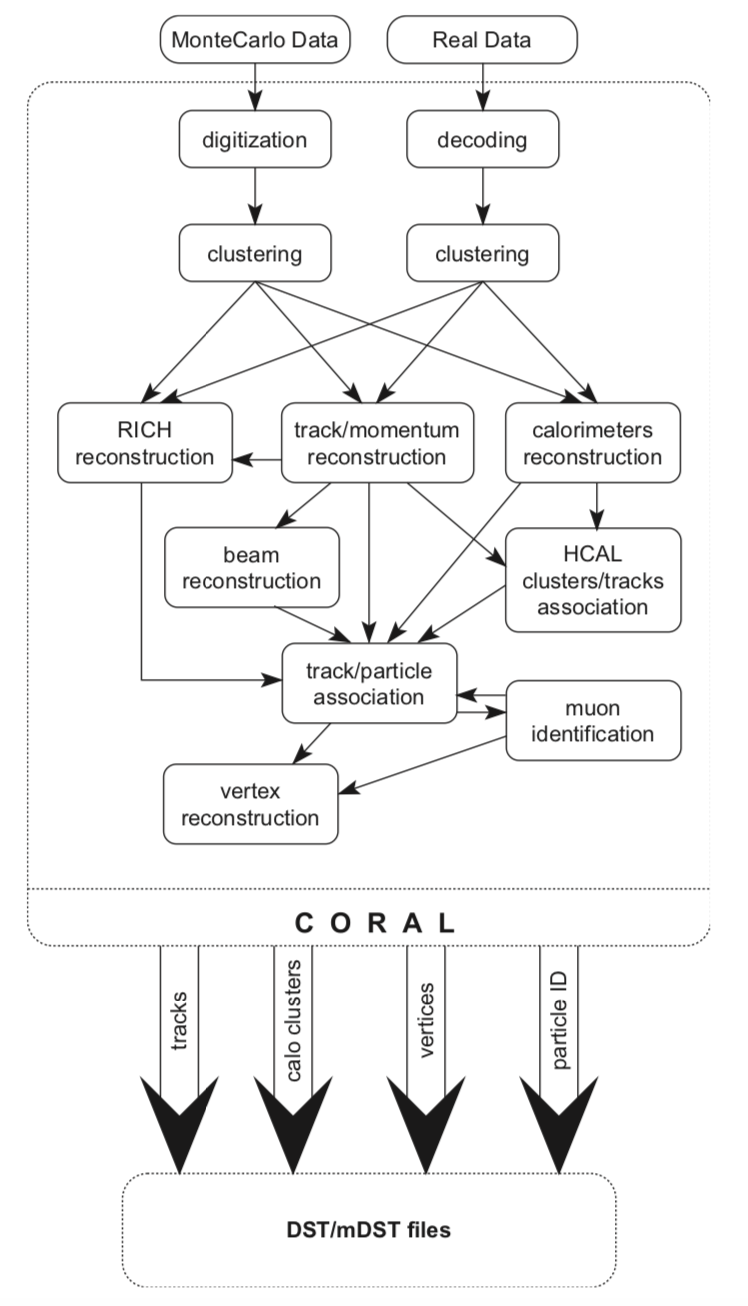
\includegraphics[scale=0.55]{./gfx/CORAL.png}
	\caption{Schematic representation of the COMPASS reconstruction software. Taken from \cite{NIM}.}
	\label{pic:CORAL}
\end{figure}
